%!TEX root = ../dynamics.tex
\section{Market Analysis}
\label{sec:market}
Finally, we study the evolution of demand vs. supply in the Amazon MTurk marketplace. We define $Demand$ as the number of new tasks published on the platform by the requesters. In addition, we compute the average reward of the tasks that were posted. Conversely, we define $Supply$ as the workforce that the crowd is providing concretized as the number of tasks that got completed in a given time window by the workers. Again, we compute the average reward of the completed tasks.


\paragraph{New Tasks Attract New Workers}
\begin{figure}[tb]
	\centering
		
\includegraphics[width=0.48\textwidth]{figures/scattermatrix}
	\caption{Scatter matrix comparing the different parameters in the demand and supply.}
	\label{fig:scatter_matrix}
\end{figure}
\begin{figure}[tb]
	\centering
		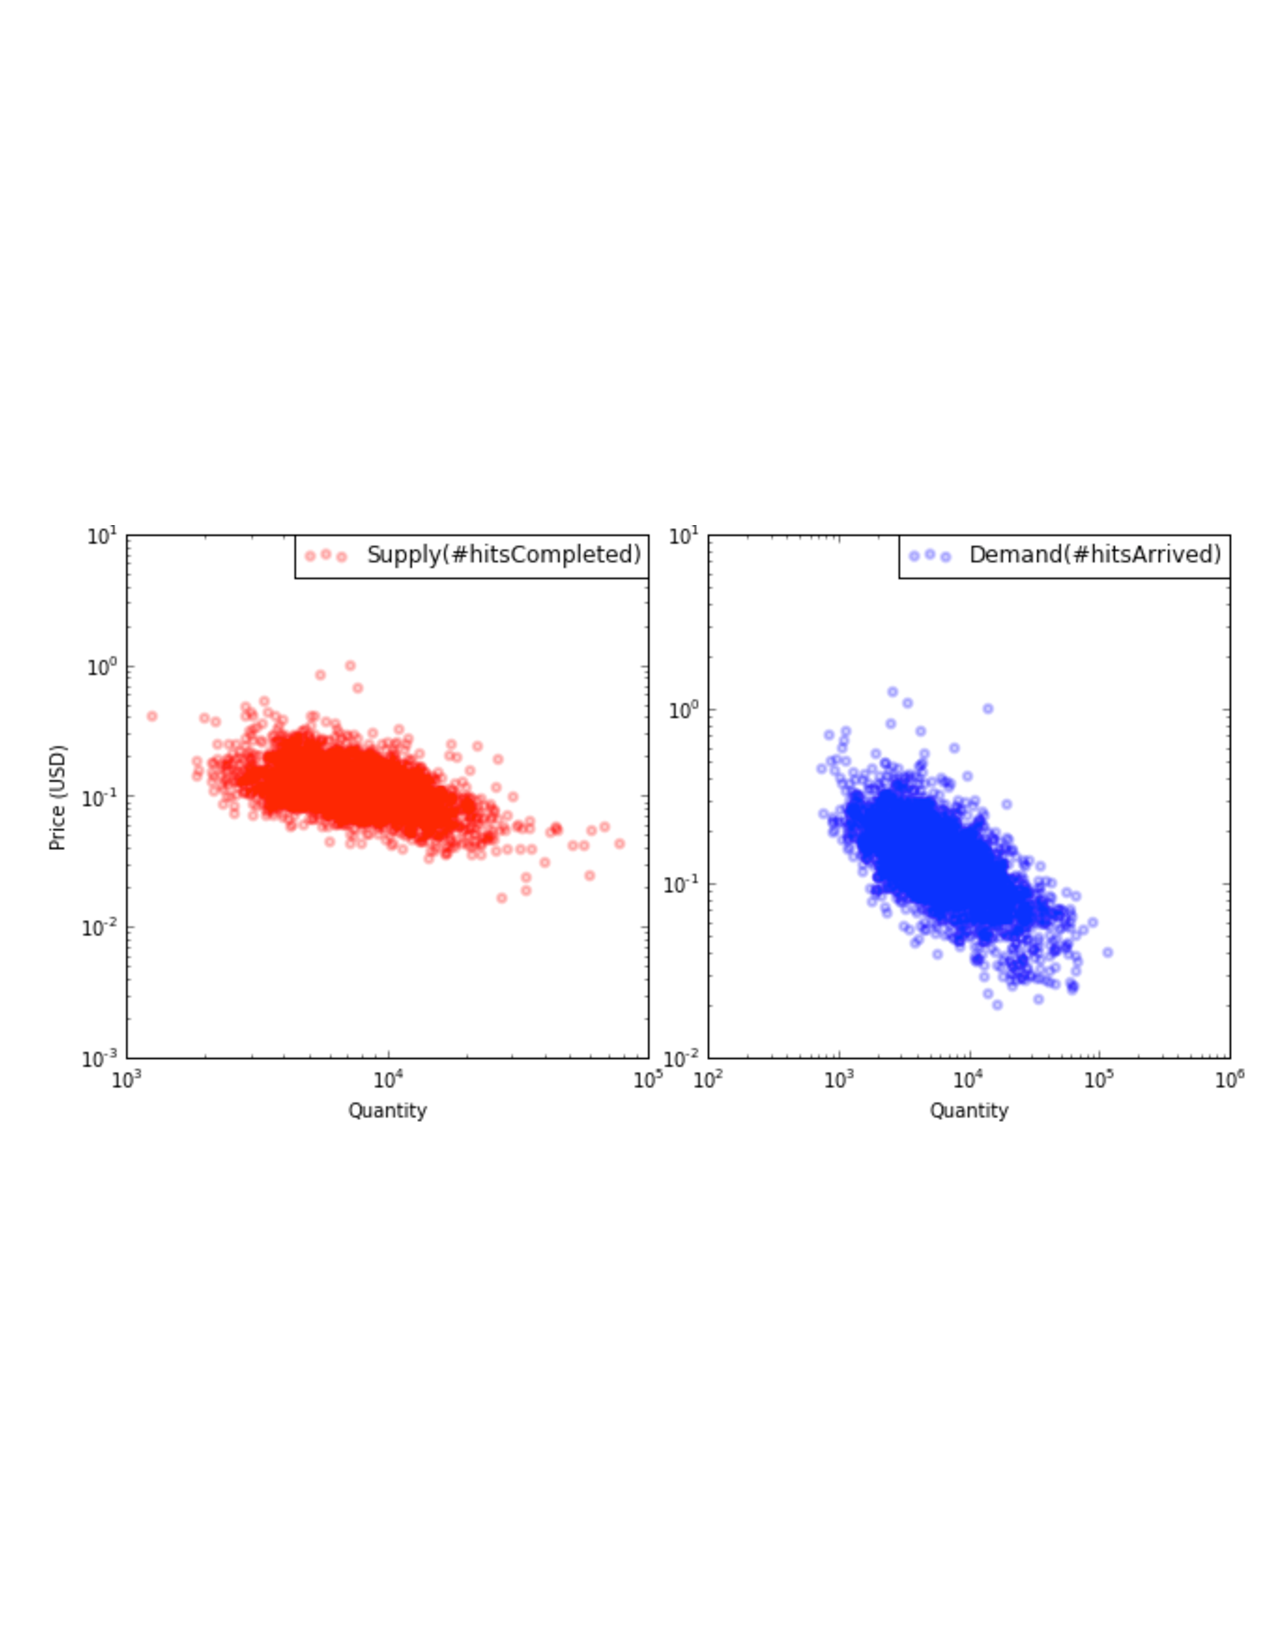
\includegraphics[width=0.48\textwidth]{figures/supply_demand}
	\caption{Supply (left) and Demand (right) versus price.}
	\label{fig:dsup}
\end{figure}
In Figure \ref{fig:scatter_matrix}, we compare the following variables: number of HITs published on the platform, average reward for such HITs, and number of HITs completed. An observation can be made about the correlation between the rewards of the number of HITs completed and those published. The results suggest that crowd workers are sensitive to newly posted tasks, and that they are constantly monitoring for new and fresh tasks. It must be noted that some workers might not be actively completing HITs on the platform but rather looking for HITs to work on by reading Web forums where other workers shared HITs. In that sense, new HITs attract new workers to the platform. This supplements our finding from Section \ref{sec:throughput}, where we showed that $start\_time$ is an important feature contributing to the throughput of a batch.  

Figure \ref{fig:dsup} (left) shows the expected relationship between supply and price: The larger the supply, the lower the price evolves, which is the usual behaviour. On the other hand, Figure \ref{fig:dsup} (right) does not match the typical demand curve (“the higher the demand the lower the price evolves”).
Instead, the demand seems to be tied to the supply (i.e., the number of new HITs completed). A possible explanation for this is the lack of bidding (or negotiation) mechanisms available to the workers; such mechanisms are not available on the current platform though they could help workers drive the prices up. 

\paragraph{New Workers Complete More Tasks}
\begin{figure}[tb]
	\centering
		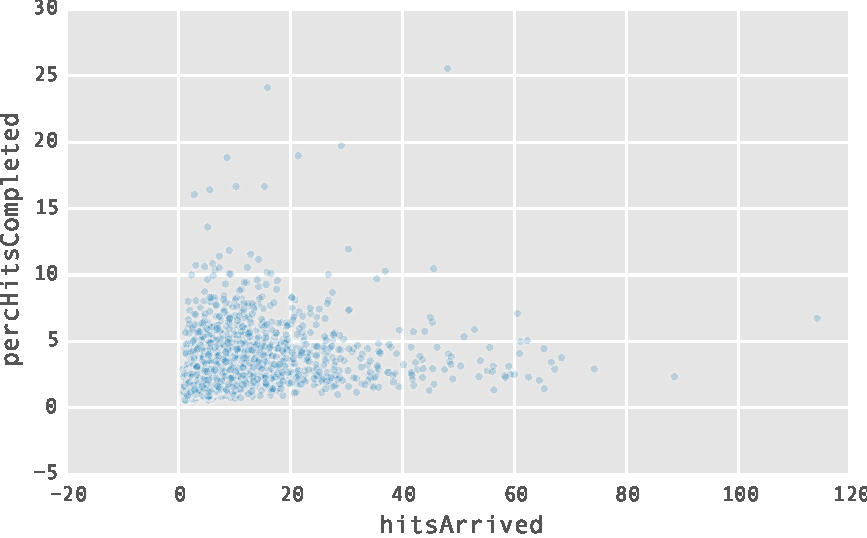
\includegraphics[width=0.48\textwidth]{figures/percHitsCompleted}
	\caption{The effect of new arrived HITs on the work  supplied.}
	\label{fig:perc_hits_completed}
\end{figure}
Along the same lines, the results detailed in Figure \ref{fig:perc_hits_completed} indicate that, as more HITs are published on the platform, a higher percentage of the available work gets done. In detail, when many HITs arrive to the platform, the overall percentage of HITs completed on the platform tends to slightly increase. As more HITs are available on the platform, an higher overall percentage indicates that many HITs are being completed. This clearly indicates that the arrival of new work also attracts new workers to the market, who also seem to spill over to other tasks (i.e., they are not just working on the fresh HITs). 

\paragraph{Weekly Periodicity}
Another behavior that we observe is the strong weekly periodicity that the demand exhibits, which is reflected by the autocorrelation that we compute on the number of available HITs as reported by Amazon Mturk (See Figure \ref{fig:autocorrelation1}). 
Figure \ref{fig:mac} shows the weekly moving average convergence divergence (MACD) of the reward attached to completed HITs. To check for periodicity effects in the amount of distributed reward we computer an autocorrelation on the time series. Figure \ref{fig:autocorrelation2} shows that there is a strong weekly periodicity effect as we observe high values in the range 0-250 hours. 

\begin{figure}[tb]
    \centering
    \begin{subfigure}[b]{0.48\textwidth}
        \centering
        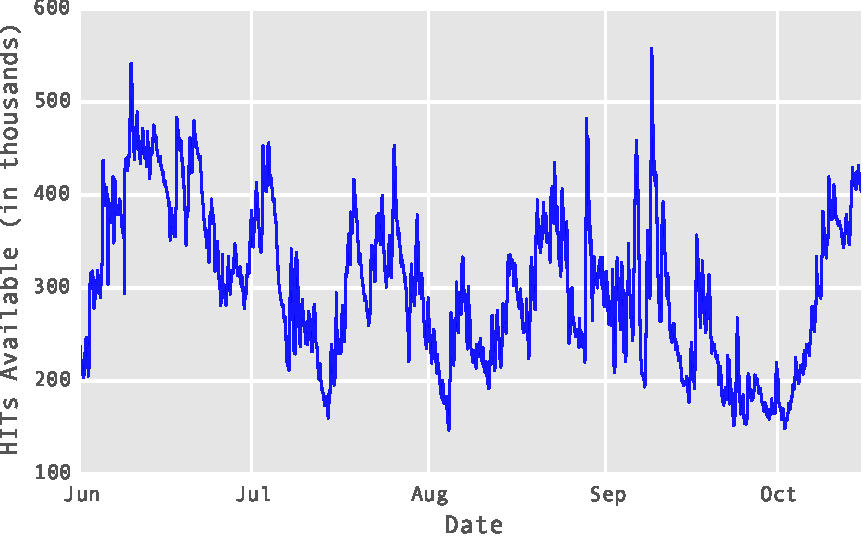
\includegraphics[width=\textwidth]{figures/out}
        \caption{HITs Available.}
        \label{fig:y equals x}
    \end{subfigure}
    \hfill
    \begin{subfigure}[b]{0.48\textwidth}
        \centering
        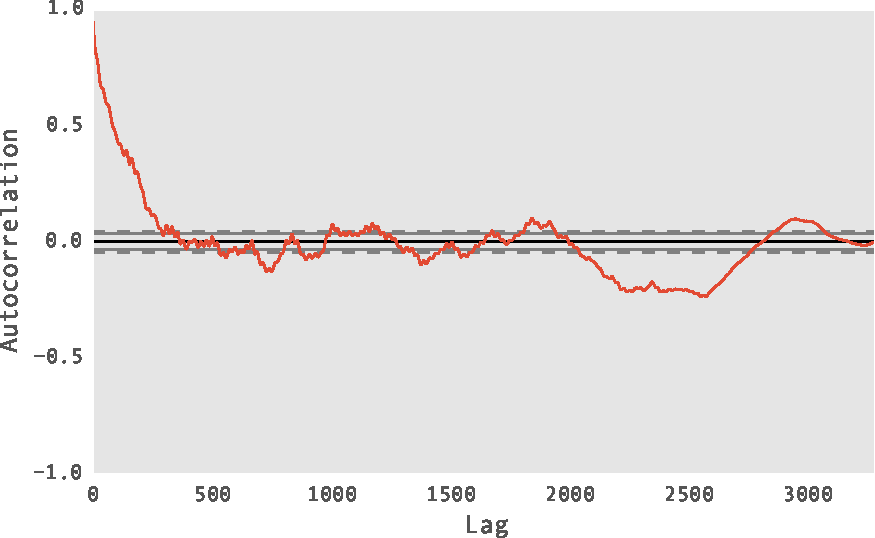
\includegraphics[width=\textwidth]{figures/out1}
        \caption{Autocorrelation.}
        \label{fig:three sin x}
    \end{subfigure}
    \hfill
    \caption{Autocorrelation of the number of HITs available on MTurk time series. There is a significant correlation that lasts 7-10 days (see left part of the graph 0-250 Hours).}
	\label{fig:autocorrelation1}
\end{figure}


\begin{figure}[tb]
    \centering
    \begin{subfigure}[b]{0.48\textwidth}
        \centering
        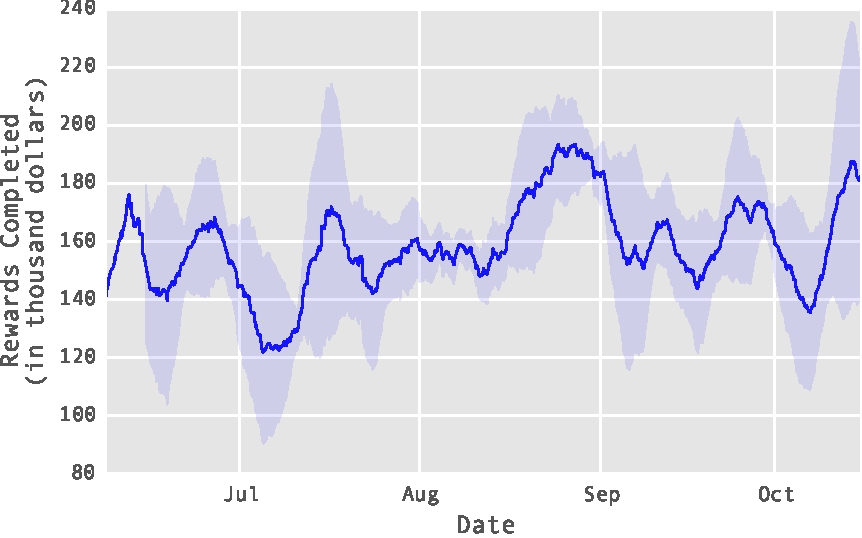
\includegraphics[width=\textwidth]{figures/mac}
        \caption{Weekly moving average on rewards completed.}
        \label{fig:mac}
    \end{subfigure}
    \hfill
    \begin{subfigure}[b]{0.48\textwidth}
        \centering
        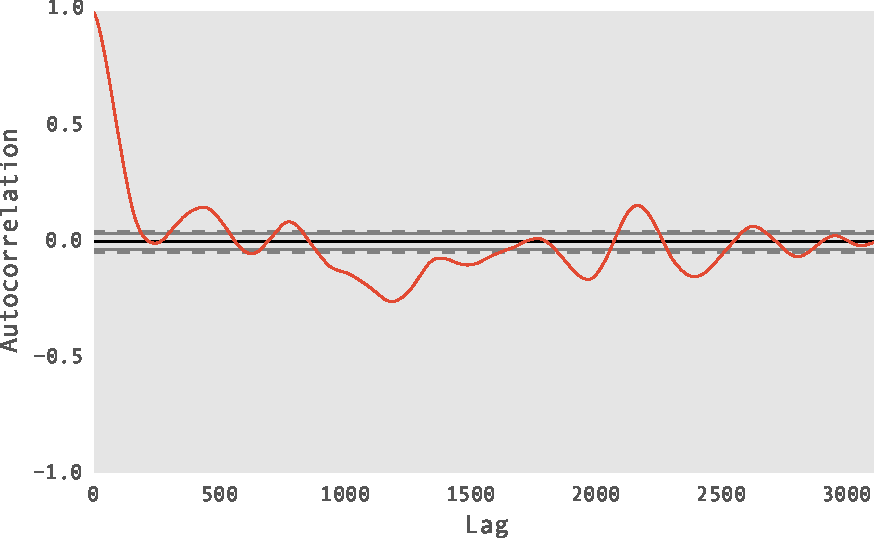
\includegraphics[width=\textwidth]{figures/macac}
        \caption{Autocorrelation.}
        \label{fig:macac}
    \end{subfigure}
    \hfill
	\caption{Autocorrelation computed on the weekly rewards moving average. Again we see a weekly periodicity (0-250 Hours).}
	\label{fig:autocorrelation2}
\end{figure}